%! TEX program = lualatex
\pdfvariable minorversion=7
\documentclass[10pt]{article}

% Packages
\usepackage[no-math]{fontspec}
\usepackage{geometry}
\usepackage{hyperref}
\usepackage[backend=biber]{biblatex} % we use the biber implementation of biblatex for bibliographies
\usepackage[nonumberlist, toc]{glossaries}
\usepackage{graphicx}
\usepackage{pdfpages}
\usepackage{booktabs}
\usepackage{float}
\usepackage{subcaption}
\usepackage{fancyhdr}
\usepackage{amsmath}
\usepackage{siunitx}

% Formatting
\geometry{letterpaper, portrait, margin=.85in}
\defaultfontfeatures{Ligatures=TeX}
\setmainfont[
    BoldFont       = Avenir Medium,
    ItalicFont     = Avenir Book Oblique,
    BoldItalicFont = Avenir Medium Oblique
]{Avenir Book}
\setmonofont{Andale Mono}
\sisetup{detect-all} % used by siunitx to always typeset units in the font of the current environment
\urlstyle{same}

\newcommand\theteamname{Midnight Sun Solar Car Team} % should not change normally
\newcommand\theuniversityname{University of Waterloo} % should also not change normally
\newcommand\theteamwebsite{www.uwmidsun.com} % should also not normally change
\newcommand\theteamphone{(519) 888-4567 x32978} % should also not normally change

\newcommand\thetitle{Electrical System Technical Report} % <--------------- add the title
\newcommand\thesubtitle{Electrical} % <--------------- add a subtitle or leave the field empty
\newcommand\theauthor{Titus Chow} % <--------------- add an author with contact info or comment this line
\newcommand\theauthorcontact{titus.chow@uwmidsun.com} % <--------------- add author's email or leave the field empty
\newcommand\thedate{\today} % <--------------- update the date, use this format

\pagestyle{fancy}
\renewcommand{\headrulewidth}{0pt}
\lhead{\thetitle}
\rhead{\theteamname}

\begin{document}

% Title Page
\begin{titlepage}
\large
\vspace*{2cm}
\centering

\includegraphics[width=.25\textwidth]{./figures/midnightSunLogoCircle.png} \\
\vspace{1.5cm}
{\LARGE \theteamname} \\
\theuniversityname \\
\vspace{2.2cm}
{\LARGE MSXII} \\
\vspace{0.4cm}
{\huge\bfseries \thetitle} \\
\vspace{0.2cm}
{\LARGE \thesubtitle} \\
\vspace{2.2cm}
\ifdefined \theauthor
\par Prepared by: \\
\theauthor \\
\theauthorcontact \\
\fi
\thedate \\
\vfill
\theteamwebsite \\
\theteamphone
\end{titlepage}

% Main Matter
\tableofcontents
\listoffigures % <-------------- uncomment for list of figures
%\listoftables % <-------------- uncomment for list of tables

\section{Overview}

Midnight Sun XII's electrical system consists of high- and low-voltage domains that are electrically isolated for safety. The high-voltage system includes the Sunpower E-series solar cells, Nomura maximum power point trackers, Tritium motor controllers and NGM SCM-150 motors. These are externally-sourced components purchased by the team and interface with the vehicle's custom embedded systems.

The low-voltage system is comprised of custom circuit-boards serving several functions for monitoring and controlling the vehicle, primarily: driver controls, power distribution, and battery management. Several smaller PCBs are located throughout the vehicle to support various sensor interfacing and data collection functions. Most boards communicate over a unified CAN bus, with some nodes supporting smaller subsystems over I2C. The low-voltage power rail is normally provided by the main battery pack via DC-DC converters, but can also be switched to an auxiliary \SI{12}{\volt} Ni-MH battery during startup or fault modes.

Due to the different CAN specifications of the Tritium WaveSculptor motor controllers, they are allocated a separate powertrain CAN network which interfaces with the primary CAN bus via dedicated transceiver boards. For similar reasons, we also allocate separate CAN buses for solar sensing and charger control.

\section{Electrical System Design}

\subsection{5.2.C.1}

\subsubsection{System Diagram}

\begin{figure}[H]
    \centering
    \includegraphics[width=\textwidth,page=4]{figures/msxii-block-diagrams}
    \caption{Block diagram of the full electrical system}
    \label{fig:msxii-electrical-full-block-diagram}
\end{figure}

\subsubsection{System Power Requirements}

Our primary power requirements are from our motors. We have two NGM SCM150s with a total peak power of 15kW and total continuous power rating of 7.5kW. We plan on limiting maximum system current to 130A, giving us plenty of headroom for our fuse.

The maximum expected current draw of our LV system is negligible, but our maximum expected peak current is around 10A with the horn and lights on. For reliability, we will use two Vicor DC-DCs in parallel with a combined current capability of 21A to power the LV system.

\subsubsection{HV Power System}

\begin{figure}[H]
    \centering
    \includegraphics[width=\textwidth,page=3]{figures/msxii-block-diagrams}
    \caption{Rough schematic of HV system with isolation mechanisms}
    \label{fig:msxii-electrical-hv-system}
\end{figure}

All HV systems are isolated at their sources by HV non-latching, normally-open relays. The main battery pack uses one relay in each enclosure to keep both enclosures disconnected when in the safe state. All other HV relays are powered by DC-DCs through Power Distribution.

In a fault condition, the main battery relay is opened, disconnecting the battery pack. This also disconnects the DC-DCs, causing all other HV relays to open.

To protect the HV system in case of a short, we are using the Eaton's Bussmann EV25-175, a DC-rated 175A High-Speed fuse capable of breaking 20kA. Per regulations, we have one in each battery enclosure. Our HV system uses 2 AWG wire rated for 255A. With a current limit set at 130A, a 175A fuse meets all fusing requirements.

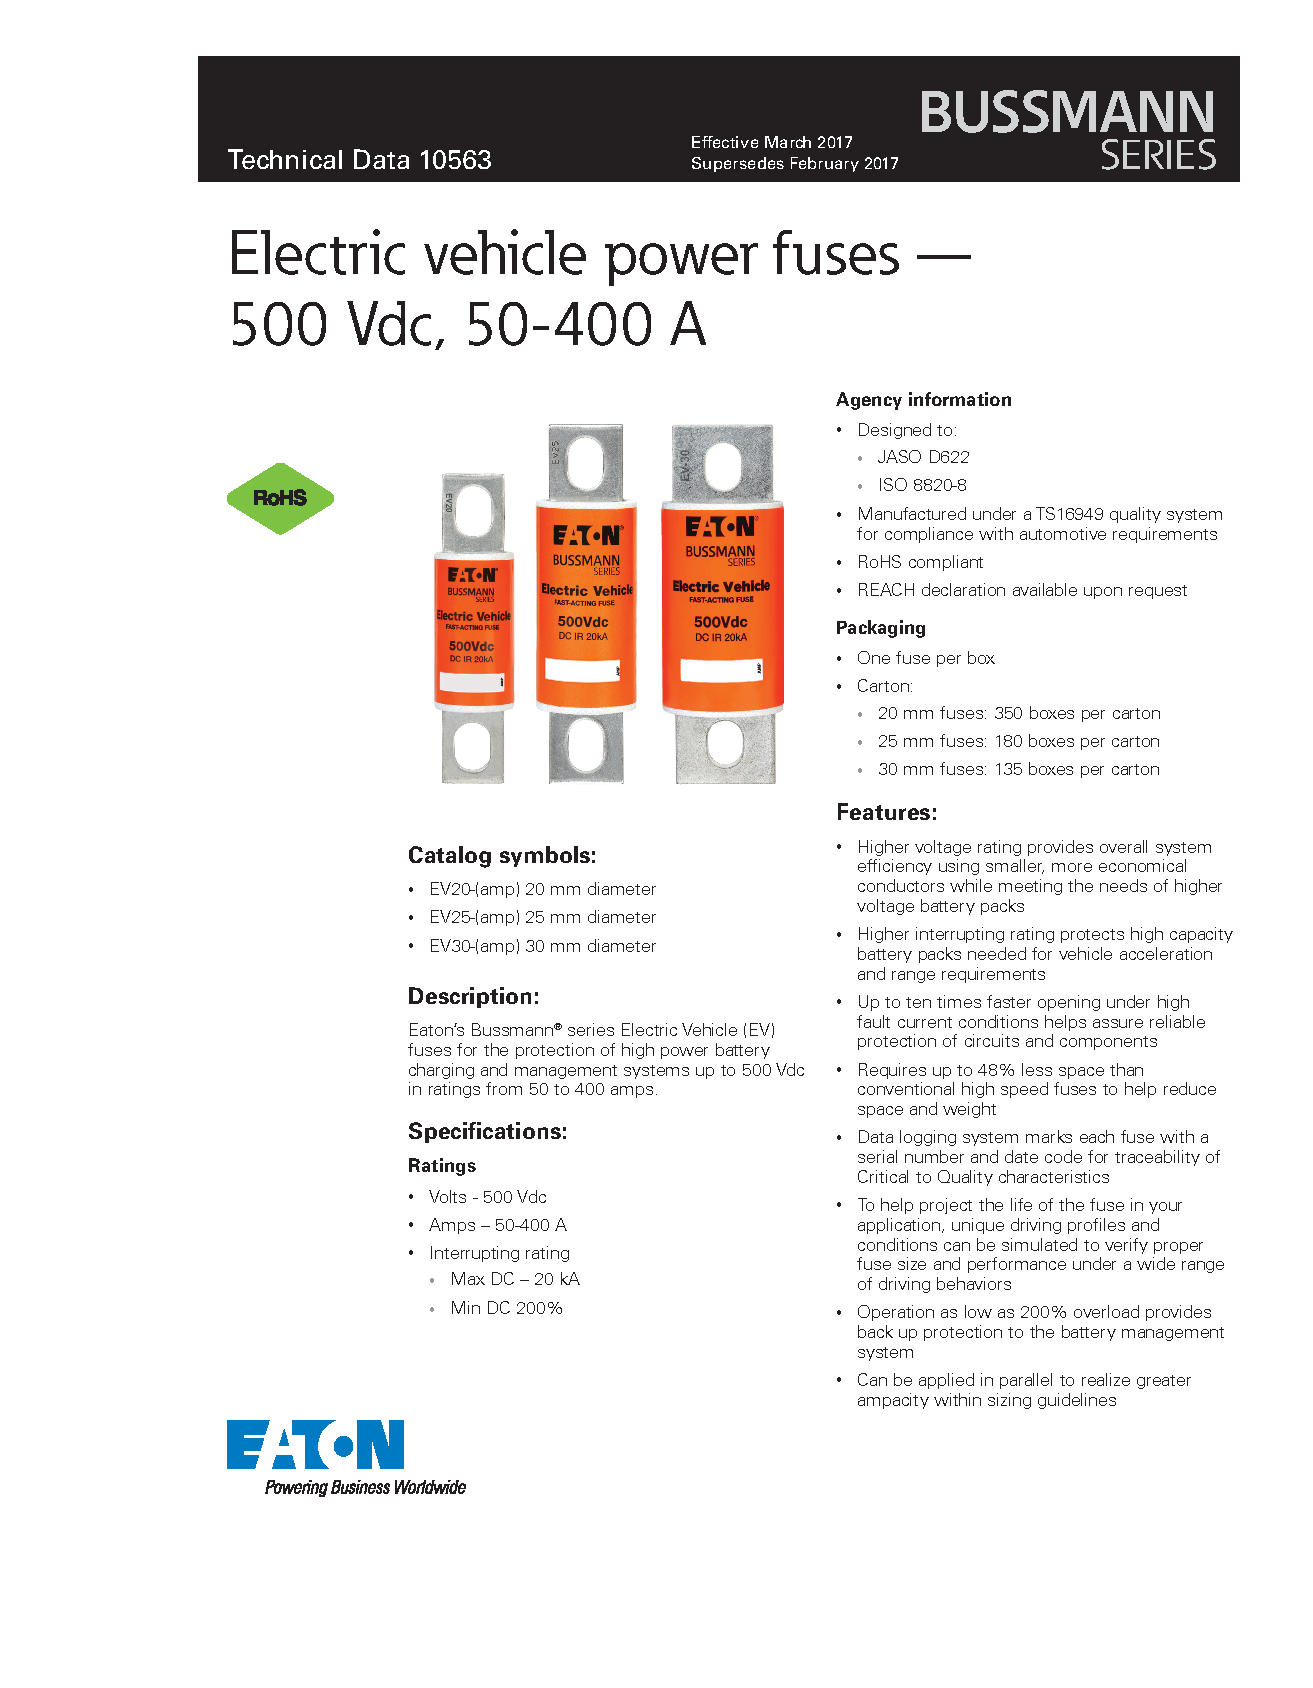
\includepdf[pages={-}]{figures/bus-ele-ds-10563-ev-power}

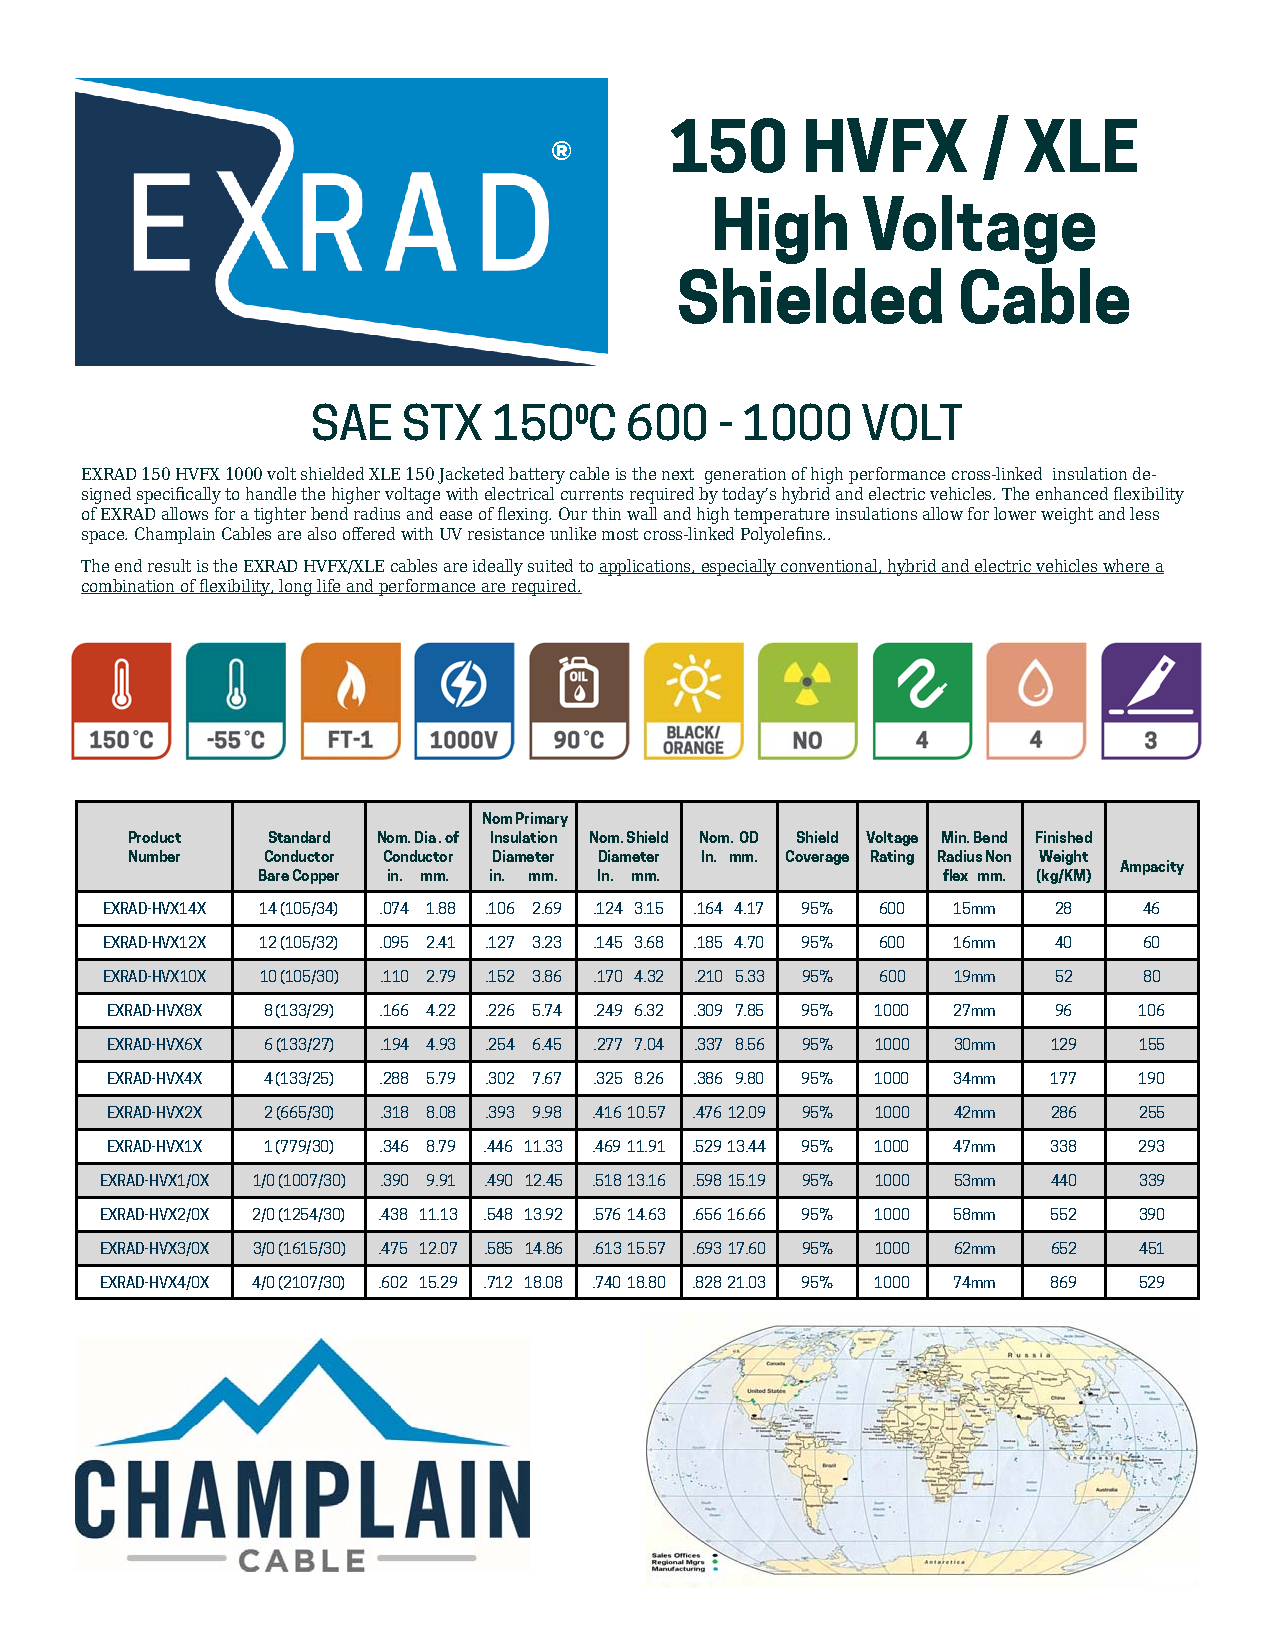
\includepdf[pages={-}]{figures/champlain-sae-exrad-150-hvfx}

\subsection{5.2.C.2}

See attached form.

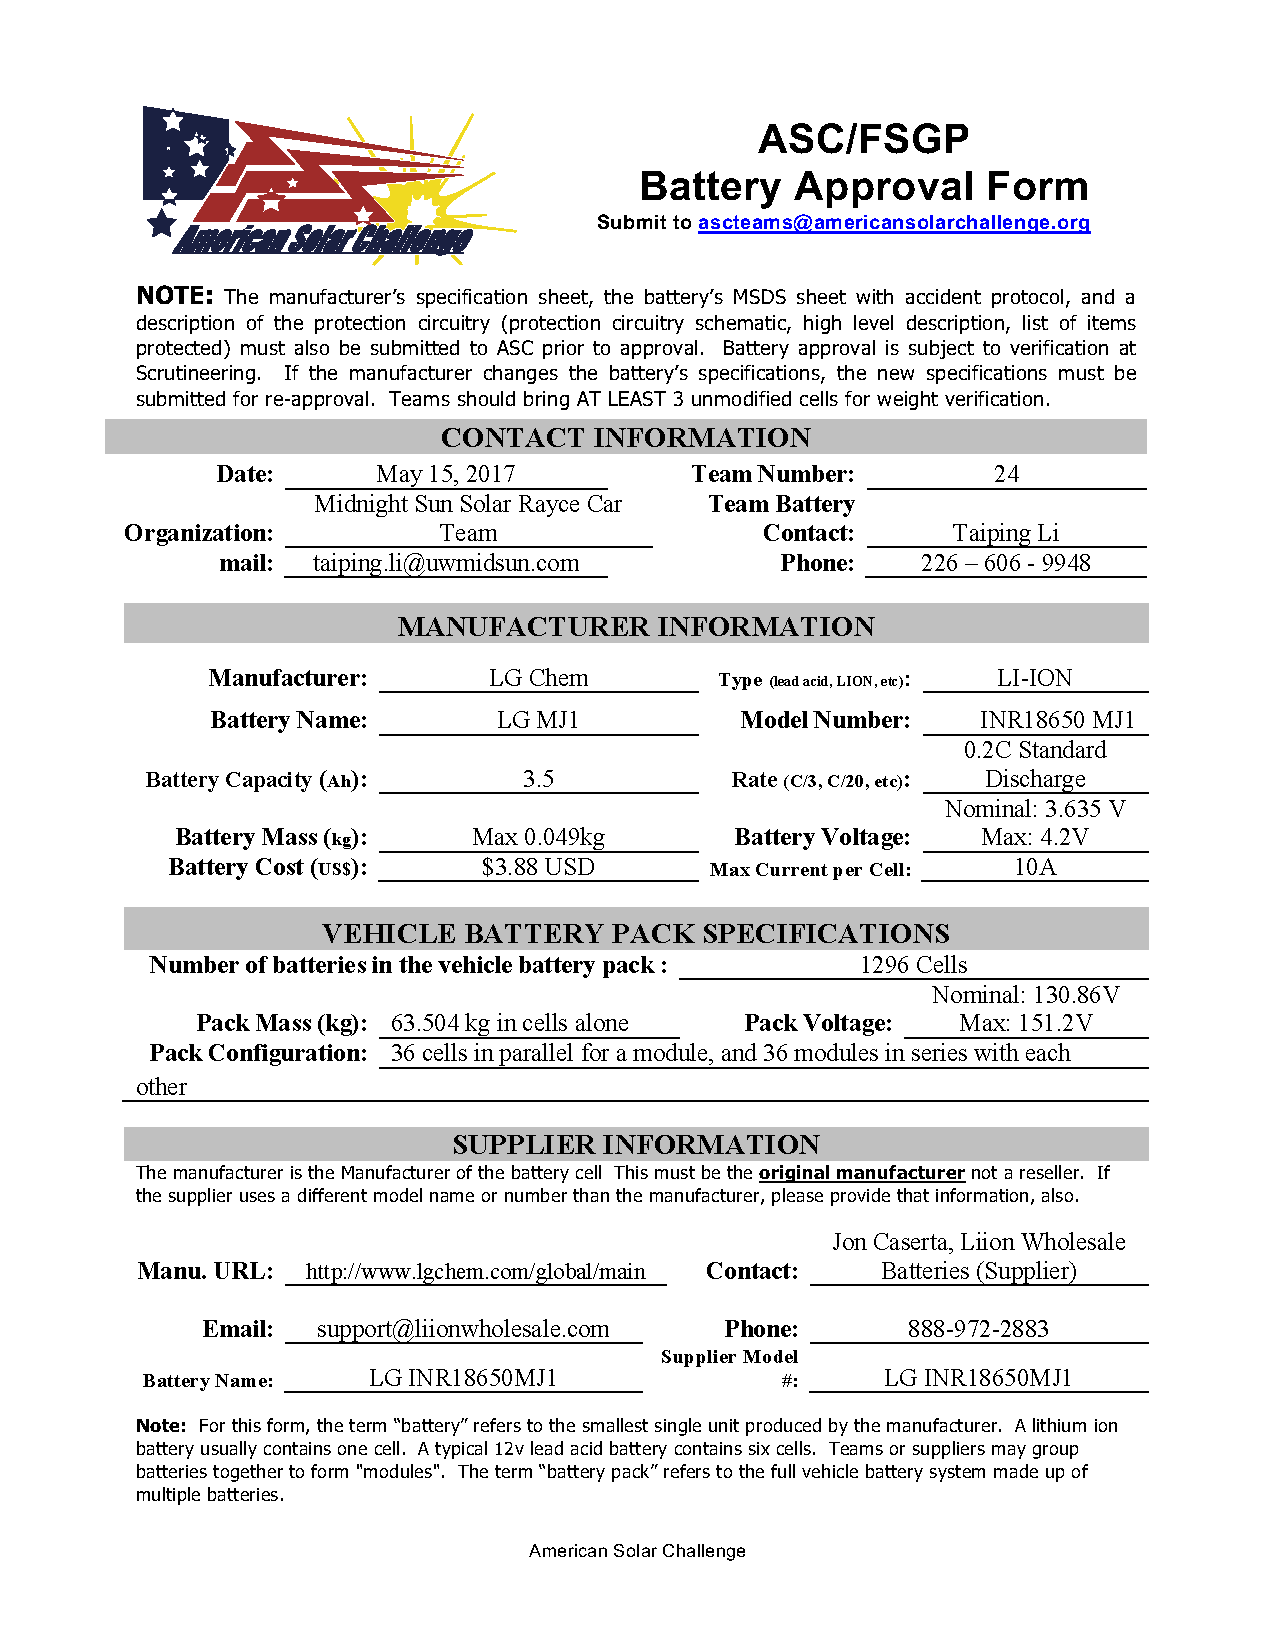
\includepdf[pages={-}]{forms/battery_approval_form.pdf}

% Bibliography
%\pagebreak
%\printbibliography

% Appendix
\pagebreak
\appendix

\end{document}
